\documentclass{beamer}
\usetheme{polimi}
\beamertemplatenavigationsymbolsempty


\usepackage{amsmath}
\usepackage{amssymb}
\usepackage{bm} % For bold math symbols
\usepackage{graphicx}
\usepackage{tikz}
\usetikzlibrary{positioning}



\usepackage{subfig} % Changed from subfigure (deprecated)
\usepackage{multirow}
\usepackage{multicol}
\usepackage{color}
\usepackage{url}
\usepackage{hyperref}
\usepackage{listings}
\usepackage[noend]{algorithm}
\usepackage{physics} 
% add image path
\graphicspath{{../Images/}}

% bibliography
\usepackage[backend=biber,style=alphabetic,sorting=none]{biblatex}
\addbibresource{mimesis.bib}


\newcommand{\supervisors}[2]{
  
    \hspace{-0.8em}
  \begin{tabular}{ll}
  \small Advisor: & \small #1 \\
  \small Co-advisor: & \small #2
  \end{tabular}
}



\DeclareMathOperator{\argmin}{argmin}
\DeclareMathOperator{\argmax}{argmax}





\title{A Modified Neural Modes Framework for\\ Soft Tissue Simulation}
\author{Andrea Bonifacio }
\date{AY: 2024-2025  \vspace{-5em} \hspace{2cm} \supervisors{Prof. Stefano Pagani}{Dr. Stéphane Cotin}
}

\begin{document}

\begin{frame}
\titlepage
\end{frame}

\begin{frame}{The problem: Soft Tissue Simulation}
    \begin{columns}[T]
        \begin{column}{0.6\textwidth}
            \begin{itemize}
                \item Soft tissue simulation is crucial in medical applications, such as computer-assisted surgery.
                \item High-fidelity simulations are computationally expensive, making real-time applications challenging.
                \item There is a strong need for fast, accurate methods that can handle large, nonlinear deformations.
            \end{itemize}
        \end{column}
        \begin{column}{0.4\textwidth}
            \begin{figure}
                \centering
                    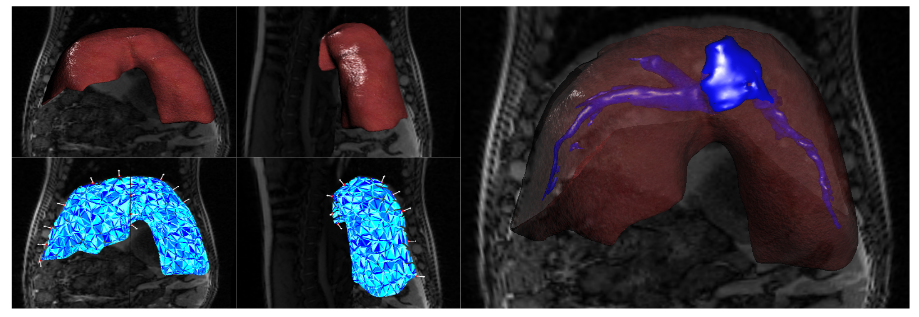
\includegraphics[width=\textwidth]{Images/liver.png}
                    \caption{Phases of the meshing process from MRI scan to obtain a digital twin of a liver. Figure from \cite{Courtecuisse_Peterlik_Trivisonne_Duriez_Cotin_2014}.}
            \end{figure}
        \end{column}
    \end{columns}
\end{frame}

\begin{frame}{Related Work}
    \begin{itemize}
        \item \textbf{MeshGraphNet} \cite{pfaffLearningMeshBasedSimulation2021a} and similar deep learning models have demonstrated impressive speedups in physical simulations.
        \item However, these models are often \textbf{black-box} in nature, and they tend to \textbf{accumulate errors} over time, leading to inaccuracies in long-term simulations.
        \item  We take inspiration from the \textbf{Neural Modes} framework \cite{Wang_Du_Coros_Thomaszewski_2024}, which tries to address these issues.
    \end{itemize}
\end{frame}


\begin{frame}{Mathematical Framework}
    \begin{columns}[T]
        \begin{column}{0.5\textwidth}
            \textbf{Neo-Hookean Model}
            \begin{itemize}
                \item A hyperelastic mechanical model designed to capture large, nonlinear deformations in soft tissues.
                \item Suitable for applications requiring accurate stress-strain relationships and volume changes.
                \item Commonly used in biomechanics and soft tissue simulations.
            \end{itemize}
        \end{column}
        
        \begin{column}{0.5\textwidth}
            \textbf{Linear Modal Analysis}
            \begin{itemize}
                \item A classical technique for simplifying dynamic systems by reducing their complexity.
                \item Focuses on dominant vibration shapes to approximate system behavior.
                \item Efficient for small deformations but struggles with nonlinear effects in large deformations.
            \end{itemize}
        \end{column}
    \end{columns}
\end{frame}

\begin{frame}{Neo-Hookean Model}
    We define the deformation of a material point \(\bm{X}\) in the reference configuration to its position \(\bm{x}(\bm{X},t)\) in the current configuration at time \(t\), and the deformation gradient \(\bm{F}\) as:
    \begin{equation}
        \bm{x}(\bm{X},t) = \bm{X} + \bm{u}(\bm{X},t), \quad \bm{F} = \frac{\partial \bm{x}}{\partial \bm{X}} = \bm{I} + \nabla_{\mathbf{X}} \bm{u}.
    \end{equation}
    
    \begin{block}{Neo-Hookean Hyperelasticity}
        We use the Neo-Hookean strain-energy density function $\Psi$,
        \begin{equation}
            \Psi(\bm{F}) = \frac{\mu}{2} (I_C - 3 - 2\ln(J)) + \frac{\lambda}{4} (J^2 - 1 - 2\ln(J)),
        \end{equation}
        where \(\mu, \lambda\) are material parameters and \(J = \det(\bm{F})\) is the volume change.
    \end{block}
\end{frame}

\begin{frame}{Neo-Hookean Model}
    The stress in the material is derived from the strain energy: \(\bm{P} = \frac{\partial \Psi}{\partial \bm{F}}\).
    
    \begin{block}{Static Problem}
        The dynamic behavior of the object is governed by the following system of PDEs, which represents the full-order model. Solving this system is accurate but computationally expensive.
        \begin{equation}
            \begin{cases}
                - \nabla_X \cdot \bm{P} = \bm{b} \quad \text{in} \quad \Omega, \\
                \bm{u} = \bm{u}_D \quad \text{on} \quad \Gamma_D, \\
                \bm{P} \cdot \bm{N} = \bm{t} \quad \text{on} \quad \Gamma_N.
            \end{cases}
        \end{equation}
        Here, \(\bm{b}\) are body forces, and the equations are subject to boundary conditions on \(\Gamma_D\) (prescribed displacement) and \(\Gamma_N\) (applied traction).
    \end{block}
\end{frame}

\begin{frame}{Neo-Hookean Model}    
    \begin{block}{Equation of Motion}
        The dynamic behavior of the object is governed by the following system of PDEs, which represents the full-order model. Solving this system is accurate but computationally expensive.
        \begin{equation}
            \begin{cases}
                \rho \frac{\partial^2 \bm{u}}{\partial t^2} - \nabla_X \cdot \bm{P} = \bm{b} \quad \text{in} \quad \Omega, \\
                \bm{u} = \bm{u}_D \quad \text{on} \quad \Gamma_D, \\
                \bm{P} \cdot \bm{N} = \bm{t} \quad \text{on} \quad \Gamma_N.
            \end{cases}
        \end{equation}
        Here, \(\rho\) is density, and the rest of the notation is as before.
    \end{block}
\end{frame}

\begin{frame}[allowframebreaks]{Modal Analysis}
    
    \begin{block}{Core Idea}
        Approximate the full deformation as a linear combination of a few dominant, low-frequency vibration shapes (modes).
    \end{block}
    
    \begin{enumerate}
        \item \textbf{Linearize System:} The nonlinear equations are linearized around the rest state (\(\bm{u}=\bm{0}\)) to get constant mass \(\bm{M}\) and stiffness \(\bm{K}\) matrices.
        \vspace{0.5em}
        
        \item \textbf{Solve Eigenvalue Problem:} We find the natural vibration modes \(\bm{\phi}_i\) and frequencies \(\omega_i\) by solving:
            \begin{equation*}
                \bm{K} \bm{\phi}_i = \omega_i^2 \bm{M} \bm{\phi}_i
            \end{equation*}
        \vspace{0.5em}
            
        \item \textbf{Modal Decomposition:} The full displacement \(\bm{u}\) is approximated using the first \(m\) modes:
            \begin{equation*}
                \bm{u}(\bm{X},t) \approx \sum_{i=1}^{m} z_i(t) \bm{\phi}_i(\bm{X})
            \end{equation*}
            We then only need to solve for the \(m\) modal coordinates \(z_i(t)\), where \(m \ll\) number of DOFs.
    \end{enumerate}
\end{frame}

\begin{frame}{The Limitation of Linear Modes}    
    \begin{alertblock}{Fundamental Problem}
        Linear modal analysis is built on a \textbf{linearization} around the undeformed state. This approximation is only valid for small deformations.
    \end{alertblock}
    
    When deformations become large:
    \begin{itemize}
        \item The model fails to capture key nonlinear effects.
        \item This leads to physically unrealistic behavior, such as incorrect volume changes and inaccurate stress distributions.
    \end{itemize}
    
    While fast, linear modes are insufficient for accurate large deformation simulation. This motivates our work to develop a method that account for nonlinearities.
\end{frame}

\begin{frame}[allowframebreaks]{Neural Modes Paper}
    The original Neural Modes framework \cite{Wang_Du_Coros_Thomaszewski_2024} introduces a novel approach to simulate nonlinear deformations by correcting the output of linear modes using a neural network. The methodology consists of the following key stages:
    
    \begin{enumerate}
        \item \textbf{Linear Modal Approximation:} The deformation is initially approximated using classical linear modal analysis, which is computationally efficient but fails to capture nonlinear effects.
        \vspace{1em}
        \item \textbf{Neural Network Correction:} A neural network is trained to learn the nonlinear corrections to the linear modal approximation. The network maps low-dimensional modal coordinates to high-dimensional corrections.
        \vspace{1em}
        \item \textbf{Self-Supervised Training:} Instead of relying on ground truth data, the network is trained by minimizing the object's internal strain energy, ensuring physically plausible corrections.
        \vspace{1em}
        \item \textbf{Dynamic Simulation:} The corrected modal approximation is used in a reduced-order dynamic solver, enabling fast simulations of large, nonlinear deformations.
    \end{enumerate}
    
    \begin{alertblock}{Key Insight}
        The self-supervised approach leverages physical principles to guide the learning process, avoiding the need for extensive labeled datasets while maintaining computational efficiency.
    \end{alertblock}
\end{frame}

\begin{frame}{Our improvements}
    Despite the promising results of the Neural Modes paper, we identified several limitations that motivated our work:
    \begin{itemize}
        \item \textbf{Limited range of deformations:} Our experiments showed that the self-supervised approach struggles with large, nonlinear deformations, leading to significant errors.
        \item \textbf{Origin penalty:} The original paper imposes a penalty on the network output to ensure that the rest state (zero modal coordinates) produces a zero correction. We employed a different approach, using bias-free layers to guarantee this property by design.
        \item \textbf{Neo-Hookean model:} The original Neural Modes framework is designed for St.Venant-Kirchhoff materials, but we needed a framework that can handle the Neo-Hookean model, which is more suitable for soft tissue simulation.
        \end{itemize}    
\end{frame}

\begin{frame}{Architectural Choice: Residual Networks (ResNets)}
    \frametitle{Architectural Choice: Residual Networks (ResNets)}
    
    We employ a Residual Network (ResNet) \cite{He_Zhang_Ren_Sun_2015}.
    
    \begin{block}{Skip Connections}
        Instead of learning a direct transformation \( \mathcal{F}(\bm{x}) \), a ResNet block learns a residual function \( \mathcal{R}(\bm{x}) \). The output is the sum of the input and the residual:
        \begin{equation*}
            \bm{x}_{\text{out}} = \bm{x}_{\text{in}} + \mathcal{R}(\bm{x}_{\text{in}})
        \end{equation*}
    \end{block}
    
    \begin{figure}
        \centering
        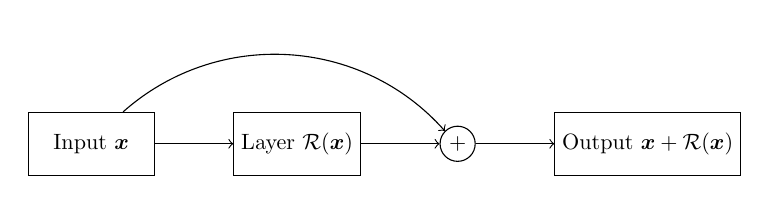
\begin{tikzpicture}[scale=0.8, every node/.style={scale=0.8}]
            \node[rectangle, draw, minimum width=2cm, minimum height=1cm] (input) at (0,0) {Input $\bm{x}$};
            \node[rectangle, draw, minimum width=2cm, minimum height=1cm, right=of input, node distance=3.5cm] (layer1) {Layer $\mathcal{R}(\bm{x})$};
            \node[circle, draw, inner sep=2pt, right=of layer1, node distance=2.5cm] (plus) {$+$};
            \node[rectangle, draw, minimum width=2.5cm, minimum height=1cm, right=of plus, node distance=2.5cm] (output) {Output $\bm{x} + \mathcal{R}(\bm{x})$};
            \draw[->] (input) -- (layer1);
            \draw[->] (layer1) -- (plus);
            \draw[->] (plus) -- (output);
            \draw[->] (input) to[bend left=45] (plus); % Skip connection
        \end{tikzpicture}
        \caption{A residual block with a skip connection.}
    \end{figure}
    

\end{frame}

\begin{frame}{Our Model: The Neural Modes Architecture}
    \frametitle{Our Model: The Neural Modes Architecture}
    
    We designed a specific ResNet to learn nonlinear deformation modes.
    
    \begin{itemize}
        \item \textbf{Input:} A low-dimensional vector of modal coordinates \( \mathbf{z} \in \mathbb{R}^{\ell_{dim}} \).
        \item \textbf{Output:} A high-dimensional nonlinear correction vector \( \bm{y} \in \mathbb{R}^{d_u} \).
    \end{itemize}
    
    The final predicted displacement is a combination of the linear modes and the learned nonlinear correction:
    \begin{equation*}
        \bm{u}_{\text{predicted}} = \underbrace{\bm{l}(\mathbf{z})}_{\text{Linear Modes}} + \underbrace{\bm{y}(\mathbf{z})}_{\text{NN Correction}}
    \end{equation*}
    
    \begin{figure}
        \centering
        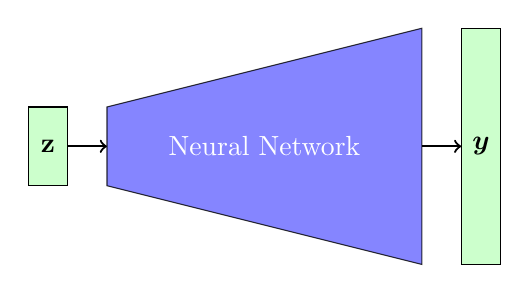
\begin{tikzpicture}
            % Modal coordinate (z)
            \draw[fill=green!20] (-3, 1) rectangle (-2.5,2);
            \node at (-2.75, 1.5) {$\mathbf{z}$}; % Label inside the rectangle
            % Displacement (y)
            \draw[fill=green!20] (2.5,0) rectangle (3,3);
            \node at (2.75, 1.5) {$\bm{y}$}; % Label inside the rectangle
            % NN mapping
            \draw[fill=blue!60,opacity=0.8] (-2,1) -- (2,-0) -- (2,3) -- (-2,2) -- cycle;
            \node[white] at (0,1.5) {Neural Network};
            % Arrow
            \draw[thick,->] (-2.5, 1.5) -- (-2, 1.5);
            \draw[thick,->] (2, 1.5) -- (2.5, 1.5);
        \end{tikzpicture}
        \caption{Neural Modes learn a mapping from low-dimensional modal coordinates \(\mathbf{z}\) to high-dimensional corrections \(\bm{y}\).}
        \label{fig:neural_modes_arch}
    \end{figure}
    
    \textbf{Key Feature:} The network is designed with bias-free layers to guarantee that an input of \(\mathbf{z}=\bm{0}\) (rest state) produces an output of \(\bm{y}=\bm{0}\), ensuring physical correctness by design.
\end{frame}

\begin{frame}{Training Strategy: Supervised Learning}
    \frametitle{Training Strategy: A Supervised, Physics-Informed Approach}
    
    While the original Neural Modes work \cite{Wang_Du_Coros_Thomaszewski_2024} used a data-free, energy-minimization approach, we adopt a supervised strategy for robustness.
    
    \begin{block}{Our Supervised Approach}
        \begin{enumerate}
            \item \textbf{Generate a Dataset:} We use a high-fidelity FEM solver to create a dataset of ground truth samples: \( (\mathbf{z}, \bm{u}_{gt}, E_{gt}) \), where:
            \begin{itemize}
                \item \( \mathbf{z} \) are the input modal coordinates.
                \item \( \bm{u}_{gt} \) is the full nonlinear ground truth displacement.
                \item \( E_{gt} \) is the ground truth internal energy.
            \end{itemize}
            \item \textbf{Train the Network:} We train the network to minimize a composite loss function that forces the prediction to match the ground truth data while respecting physical laws.
        \end{enumerate}
    \end{block}
    
    \begin{alertblock}{Advantage}
        This supervised method avoids difficult energy landscapes and ensures the network learns from physically valid, large-deformation examples, leading to better generalization.
    \end{alertblock}
\end{frame}

\begin{frame}{The Loss Function: Blending Data and Physics}
    \frametitle{The Loss Function: Blending Data and Physics}
    
    Our total loss function is a weighted sum of four components:
    \begin{equation*}
        \mathcal{L} = \alpha_1 \mathcal{L}_E + \alpha_2 \mathcal{L}_u + \gamma_1 \mathcal{L}_{ortho} + \gamma_2 \mathcal{L}_{BC}
    \end{equation*}
    
    \begin{description}
        \item[\(\mathcal{L}_u\) (Displacement Loss)] The primary supervised signal. Enforces that the predicted displacement matches the FEM ground truth.
        \begin{equation*}
            \mathcal{L}_u = \text{MSE}(\bm{X} + \bm{l} + \bm{y}, \quad \bm{u}_{gt})
        \end{equation*}
        
        \item[\(\mathcal{L}_E\) (Energy Loss)] A physics-informed term. Ensures the predicted configuration has the correct internal strain energy (compared on a log scale for stability).
        \begin{equation*}
            \mathcal{L}_E = \text{MSE}(\log_{10}(E_{pred}), \quad \log_{10}(E_{gt}))
        \end{equation*}
        
        \item[\(\mathcal{L}_{ortho}\) (Orthogonality Loss)] A geometric constraint ensuring the nonlinear correction \(\bm{y}\) is orthogonal to the linear displacement \(\bm{l}\).
        
        \item[\(\mathcal{L}_{BC}\) (Boundary Loss)] A physical constraint that penalizes any violation of fixed boundary conditions.
    \end{description}
\end{frame}

\begin{frame}{Data Generation via Modal Forces}
    \frametitle{Data Generation via Modal Forces}
    
    To create a meaningful training dataset, we need physically plausible deformations.
    
    \begin{block}{Problem}
        How do we generate external forces that produce a rich and relevant set of deformations?
    \end{block}
    
    \begin{block}{Our Solution: Modal Forces}
        \begin{enumerate}
            \item We linearize the system at rest to get the stiffness matrix \(\mathbb{K}\).
            
            \item We perform an eigenvalue decomposition of \(\mathbb{K}\) to find the deformation modes \(\boldsymbol{\Phi}\).
            
            \item We generate external forces as a linear combination of these modes:
            \begin{equation*}
                \bm{f}^{ext} = \boldsymbol{\Phi} \bm{q}
            \end{equation*}
            where \(\bm{q}\) is a vector of modal force coefficients that we can control.
            
            \item We apply these physically-grounded forces \(\bm{f}^{ext}\) to the \textbf{full nonlinear FEM solver} to compute the ground truth displacement \(\bm{u}_{gt}\) and energy \(E_{gt}\).
        \end{enumerate}
    \end{block}
    
    This ensures our training data is based on the object's natural deformation patterns.
\end{frame}

\begin{frame}{The Importance of Realistic Sampling}
    \frametitle{The Importance of Realistic Sampling}
    
    \begin{columns}[T]
        \begin{column}{0.5\textwidth}
            \textbf{Problem: Random Sampling}
            
            Simply picking random modal coordinates \(\mathbf{z}\) often results in physically implausible, high-energy configurations.
            
            \begin{figure}
                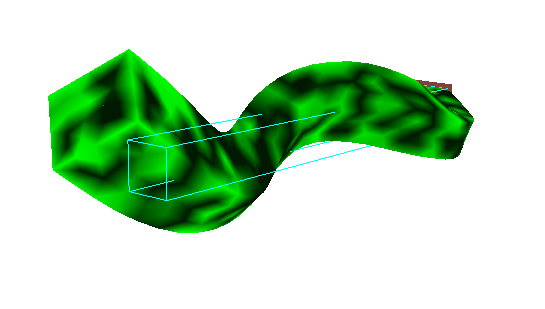
\includegraphics[width=\textwidth]{Images/z_random.png}
                \caption{Unnatural deformation from random sampling of high-frequency modes.}
                \label{fig:bad_sampling}
            \end{figure}
        \end{column}
        
        \begin{column}{0.5\textwidth}
            \textbf{Solution: Structured Data Generation}
            
            Our modal force approach generates deformations that are:
            \begin{itemize}
                \item Physically plausible.
                \item Energetically favorable.
                \item Cover the most important deformation patterns of the object.
            \end{itemize}
            
            \vspace{2em}
            This ensures the network is trained on meaningful examples, leading to a more robust and accurate model.
        \end{column}
    \end{columns}
\end{frame}

\begin{frame}{Application: Fast Dynamic Simulation}
    \frametitle{Application: Fast Dynamic Simulation}
    
    Once trained, the Neural Modes network enables rapid dynamic simulations.
    
    \begin{block}{Process at Each Time Step}
        Instead of solving a large, computationally expensive FEM problem, we solve a small optimization problem in the low-dimensional modal space. We find the next set of modal coordinates \(\mathbf{z}_{n+1}\) by minimizing the total energy of the system:
        
        \begin{equation}
            \mathbf{z}_{n+1} = \underset{\mathbf{z}}{\argmin} \underbrace{\frac{1}{2h^2} \|\bm{n}(\mathbf{z}) - 2\bm{u}_n + \bm{u}_{n-1}\|_{\bm{M}}^2}_{\text{Inertial Term (Implicit Euler)}} + \underbrace{\mathcal{E}(\bm{n}(\mathbf{z}))}_{\text{Potential Energy}}
        \end{equation}
        where \(\bm{n}(\mathbf{z})\) is the full displacement predicted by our Neural Modes model.
    \end{block}
    
    \begin{alertblock}{Result}
        This approach drastically reduces the computational cost per time step, making real-time simulation of large, nonlinear deformations feasible.
    \end{alertblock}
\end{frame}


\begin{frame}{Numerical Experiments: Setup}
    \frametitle{Numerical Experiments: Setup and Test Cases}
    
    We validate our method on two 3D geometries with soft tissue properties ($E = 10^6$ Pa, $\nu = 0.45$).
    
    \begin{columns}[T]
        \begin{column}{0.45\textwidth}
            \textbf{1. Cantilever Beam}
            \begin{itemize}
                \item A classic structural benchmark.
                \item Simple, well-understood deformation modes (bending, torsion).
                \item Ideal for initial validation.
                \item Discretized with ~800 tetrahedral elements.
            \end{itemize}
        \end{column}
        
        \begin{column}{0.55\textwidth}
            \textbf{2. Stanford Bunny} \cite{bunny-mesh}
            \begin{itemize}
                \item A complex, realistic geometry.
                \item Tests robustness and generalization.
                \item Irregular shape leads to coupled, intricate deformation modes.
                \item Discretized with ~22,000 tetrahedral elements.
            \end{itemize}
            \begin{figure}
                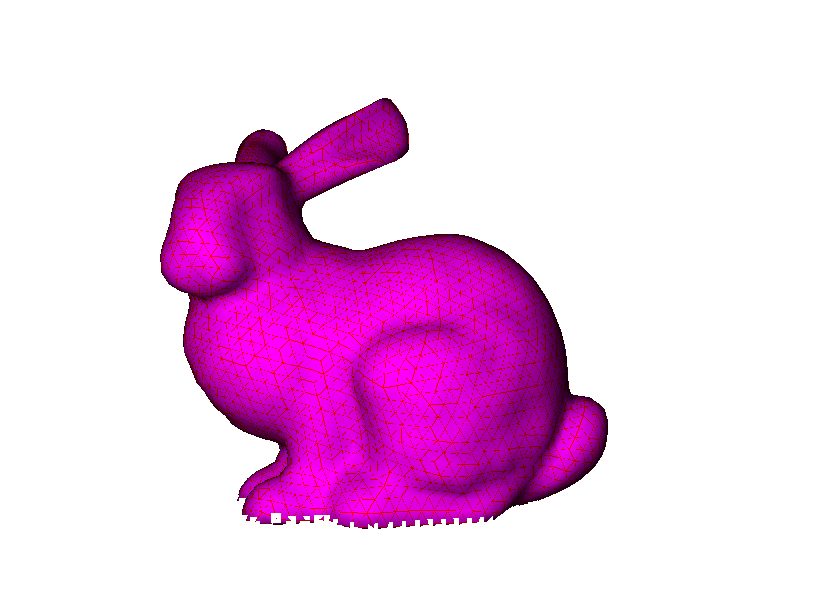
\includegraphics[width=0.6\textwidth]{Images/stanford_bunny.png}
            \end{figure}
        \end{column}
    \end{columns}
    
    \begin{alertblock}{Optimal Number of Modes}
        An initial analysis showed that using \textbf{7 modes} provides a good balance between accuracy and model complexity, achieving a displacement error below $10^{-3}$.
    \end{alertblock}
\end{frame}

\begin{frame}{Training and Model Justification}
    \frametitle{Training and Justification for Supervised Learning}
    
    We trained our model using a supervised approach on datasets of 600 (beam) and 500 (bunny) FEM simulations.
    
    \begin{columns}[T]
        \begin{column}{0.5\textwidth}
            \textbf{Training Loss (Beam)}
            \begin{itemize}
                \item The model learns quickly, with the loss dropping significantly in the first few epochs.
                \item Training was stable over 200 epochs, indicating good generalization.
            \end{itemize}
            \begin{figure}
                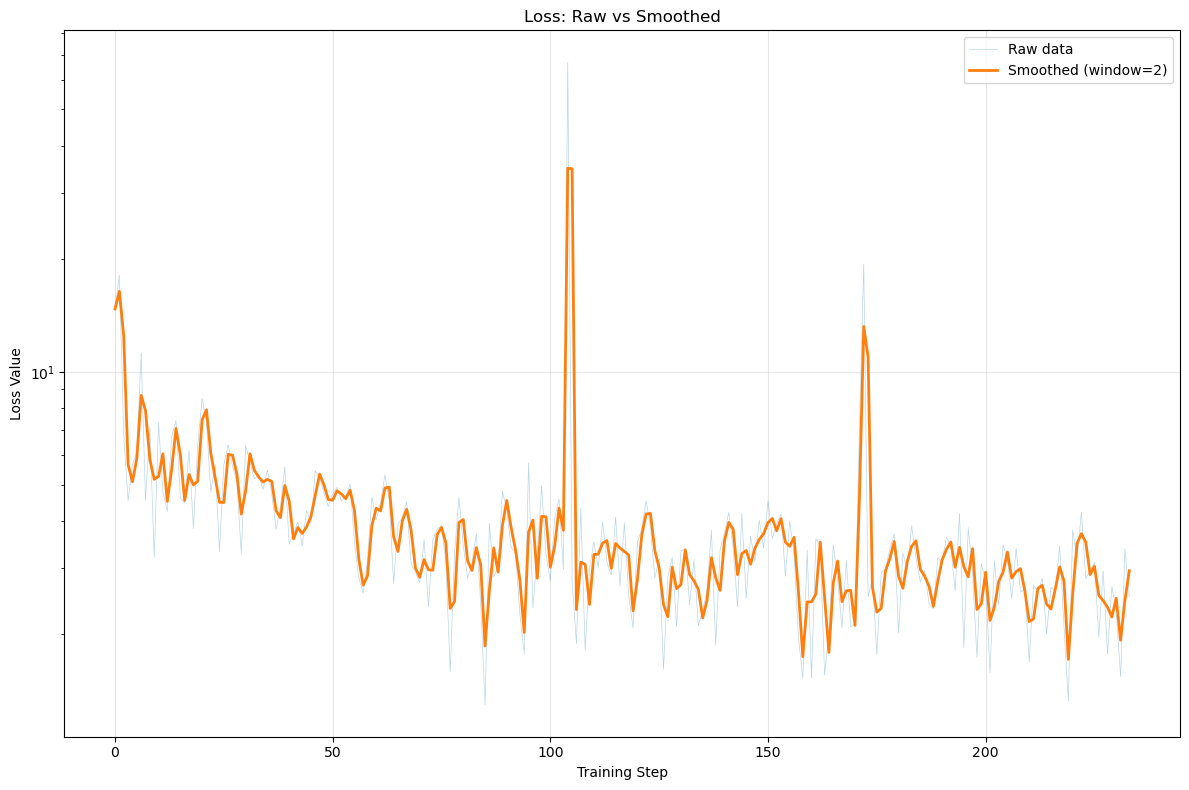
\includegraphics[width=\textwidth]{Images/training_loss_smoothed_logy.png}
                \caption{Total training loss.}
            \end{figure}
        \end{column}
        
        \begin{column}{0.5\textwidth}
            \textbf{Why not self-supervised?}
            We tested the data-free, energy-minimization approach from prior work \cite{Wang_Du_Coros_Thomaszewski_2024}.
            \begin{itemize}
                \item \textbf{Result:} The self-supervised model performed no better than simple linear modes.
            \end{itemize}
            \begin{figure}
                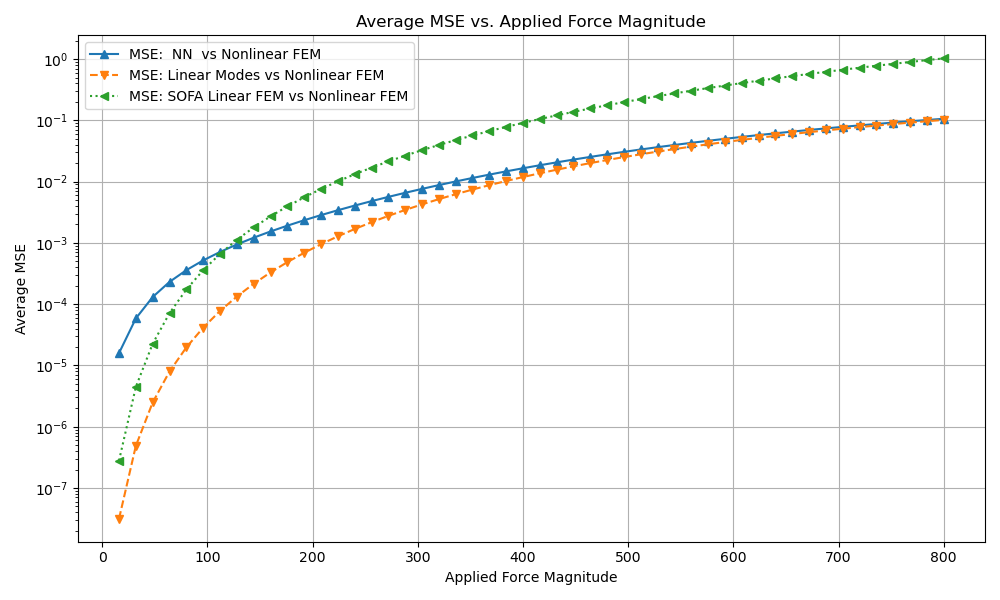
\includegraphics[width=\textwidth]{Images/self_supervised_mse.png}
                \caption{Self-supervised (blue) vs. Linear Modes (orange).}
            \end{figure}
            \textbf{Conclusion:} A supervised approach is necessary for this problem to achieve high accuracy.
        \end{column}
    \end{columns}
\end{frame}

\begin{frame}{Static Validation: Cantilever Beam}
    \frametitle{Static Validation: Cantilever Beam}
    
    We compared our Neural Modes (NM) against Linear Modes (LM) and Linear FEM using the nonlinear FEM solution as ground truth.
    
    \begin{columns}[T]
        \begin{column}{0.5\textwidth}
            \textbf{Displacement Error (MSE)}
            \begin{itemize}
                \item For small forces, LM is accurate.
                \item For large, nonlinear deformations, \textbf{NM is an order of magnitude more accurate} than both linear methods.
            \end{itemize}
            \begin{figure}
                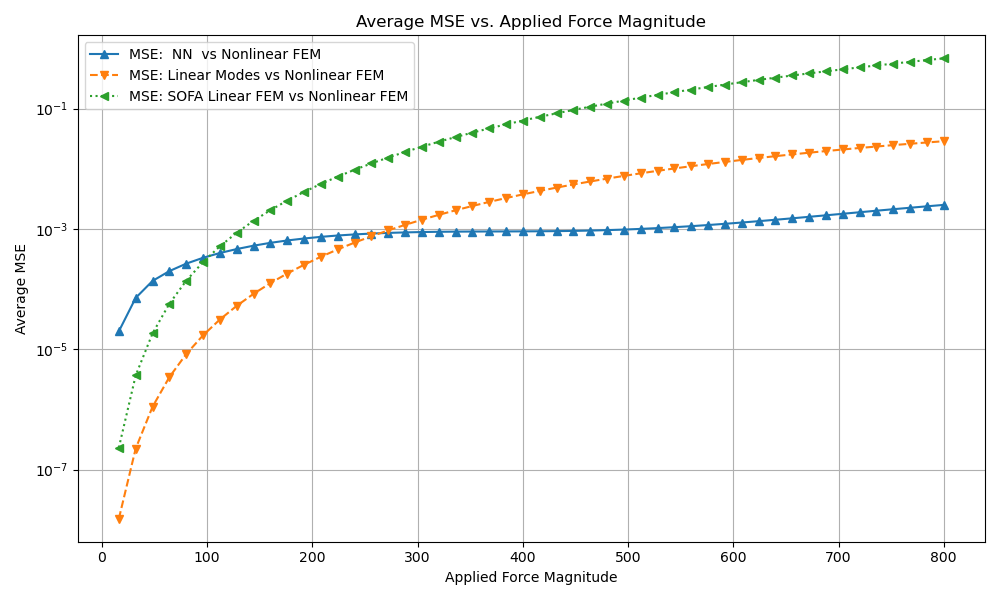
\includegraphics[width=\textwidth]{Images/beam_static_mse.png}
                \caption{Average MSE vs. Applied Force.}
            \end{figure}
        \end{column}
        
        \begin{column}{0.5\textwidth}
            \textbf{Internal Energy}
            \begin{itemize}
                \item The energy of the linear models diverges significantly from the ground truth under large deformation.
                \item Our \textbf{NM model predicts physically realistic energy levels}, closely matching the ground truth.
            \end{itemize}
            \begin{figure}
                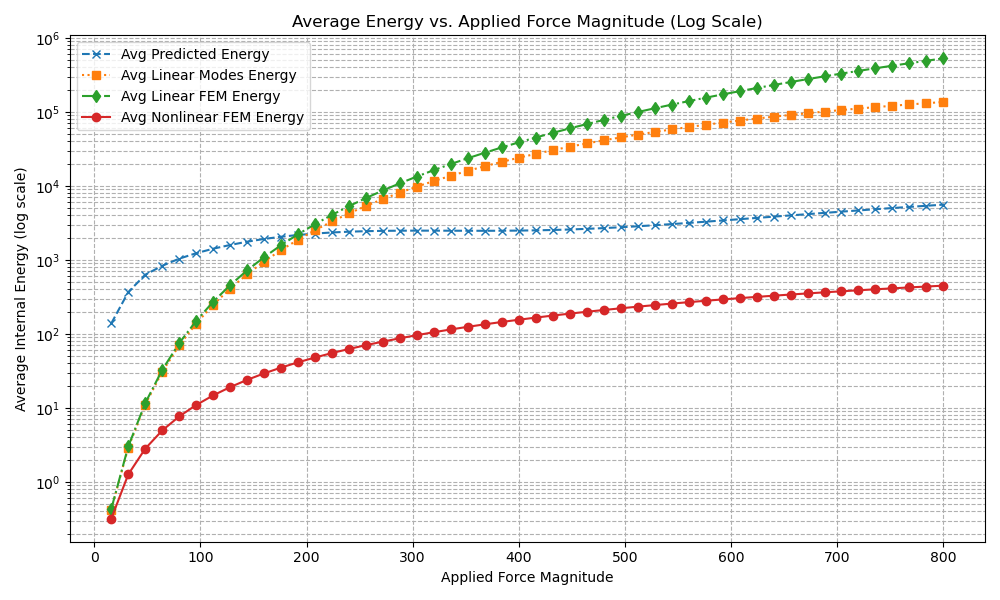
\includegraphics[width=\textwidth]{Images/beam_static_energy.png}
                \caption{Internal Energy vs. Applied Force.}
            \end{figure}
        \end{column}
    \end{columns}
\end{frame}

\begin{frame}{Static Validation: Stanford Bunny}
    \frametitle{Static Validation: Stanford Bunny}
    
    The same trend holds for the complex bunny geometry, where nonlinear effects are even more pronounced.
    
    \begin{columns}[T]
        \begin{column}{0.5\textwidth}
            \textbf{Displacement Error (MSE)}
            \begin{itemize}
                \item The NM model again shows a significant accuracy improvement of nearly an order of magnitude in the nonlinear regime.
            \end{itemize}
            \begin{figure}
                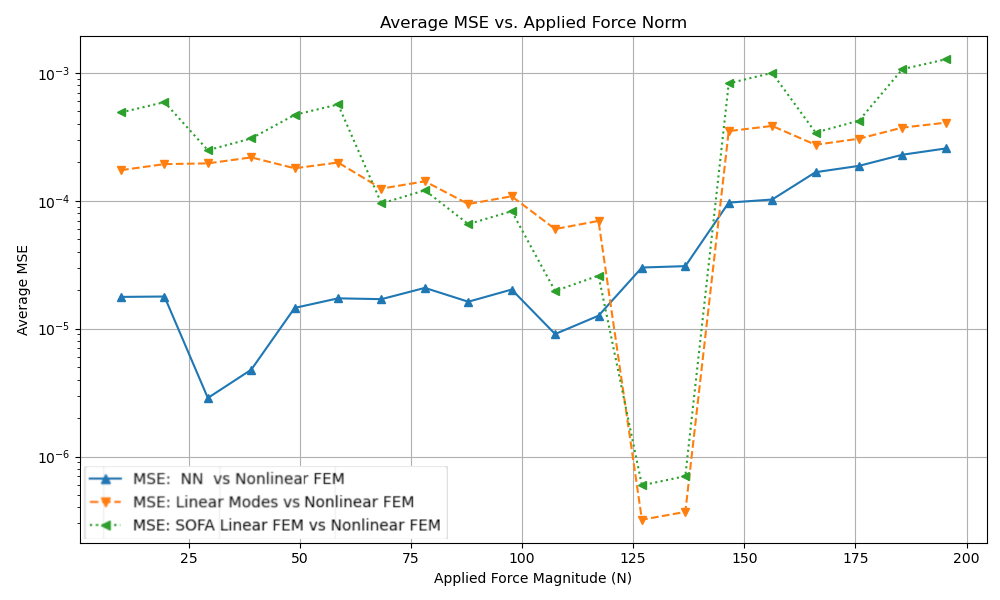
\includegraphics[width=\textwidth]{Images/bunny_static_mse.png}
                \caption{Average MSE vs. Applied Force.}
            \end{figure}
        \end{column}
        
        \begin{column}{0.5\textwidth}
            \textbf{Internal Energy}
            \begin{itemize}
                \item The energy metric is crucial for the bunny, as much of the body does not deform.
                \item Linear models have energy errors of \textbf{two+ orders of magnitude}, while our NM model remains close to the ground truth.
            \end{itemize} 
            \begin{figure}
                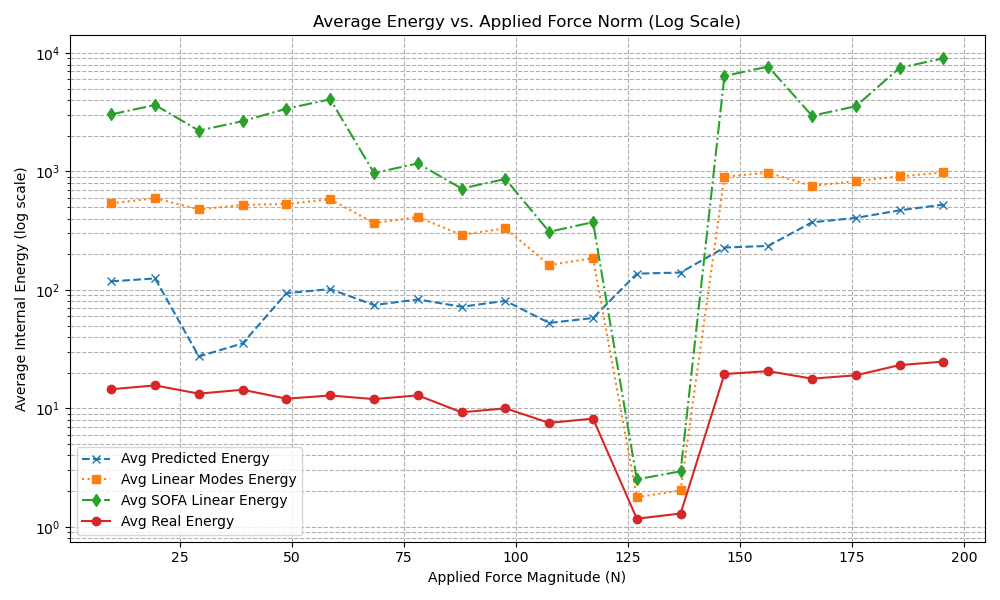
\includegraphics[width=\textwidth]{Images/bunny_static_energy.png}
                \caption{Internal Energy vs. Applied Force.}
            \end{figure}
        \end{column}
    \end{columns}
\end{frame}

\begin{frame}{Qualitative Results and Interpretability}
    \frametitle{Qualitative Results and Interpretability}
    
    \begin{columns}[T]
        \begin{column}{0.4\textwidth}
            \textbf{Visual Comparison}
            \begin{itemize}
                \item Our model (\textcolor{magenta}{magenta}) closely matches the ground truth (\textcolor{green!50!black}{green}).
                \item Linear models (\textcolor{red}{red wireframe}) fail to capture the large, nonlinear bending.
            \end{itemize}
            \begin{figure}
                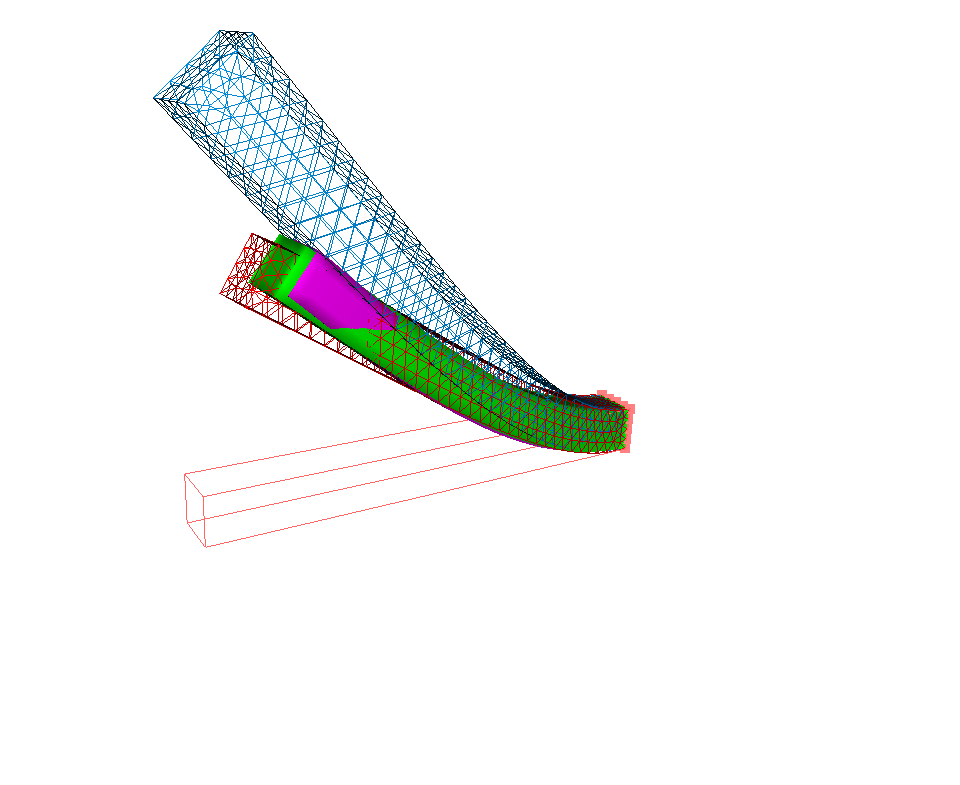
\includegraphics[width=\textwidth]{Images/sofa_example_beam.png}
                \caption{Cantilever Beam}
            \end{figure}
            \begin{figure}
                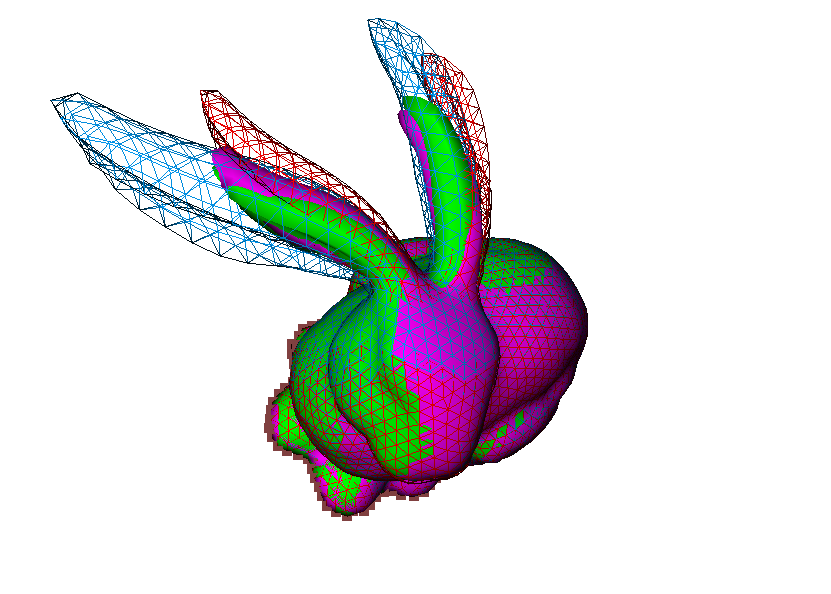
\includegraphics[width=\textwidth]{Images/sofa_example_bunny.png}
                \caption{Stanford Bunny}
            \end{figure}
        \end{column}
        
        \begin{column}{0.6\textwidth}
            \textbf{Interpretability}
            \begin{itemize}
                \item Unlike a pure black-box model, our framework is interpretable.
                \item We can visualize how the network learns to correct each individual linear mode.
                \item This provides physical insight into the learned nonlinearities.
            \end{itemize}
            \begin{figure}
                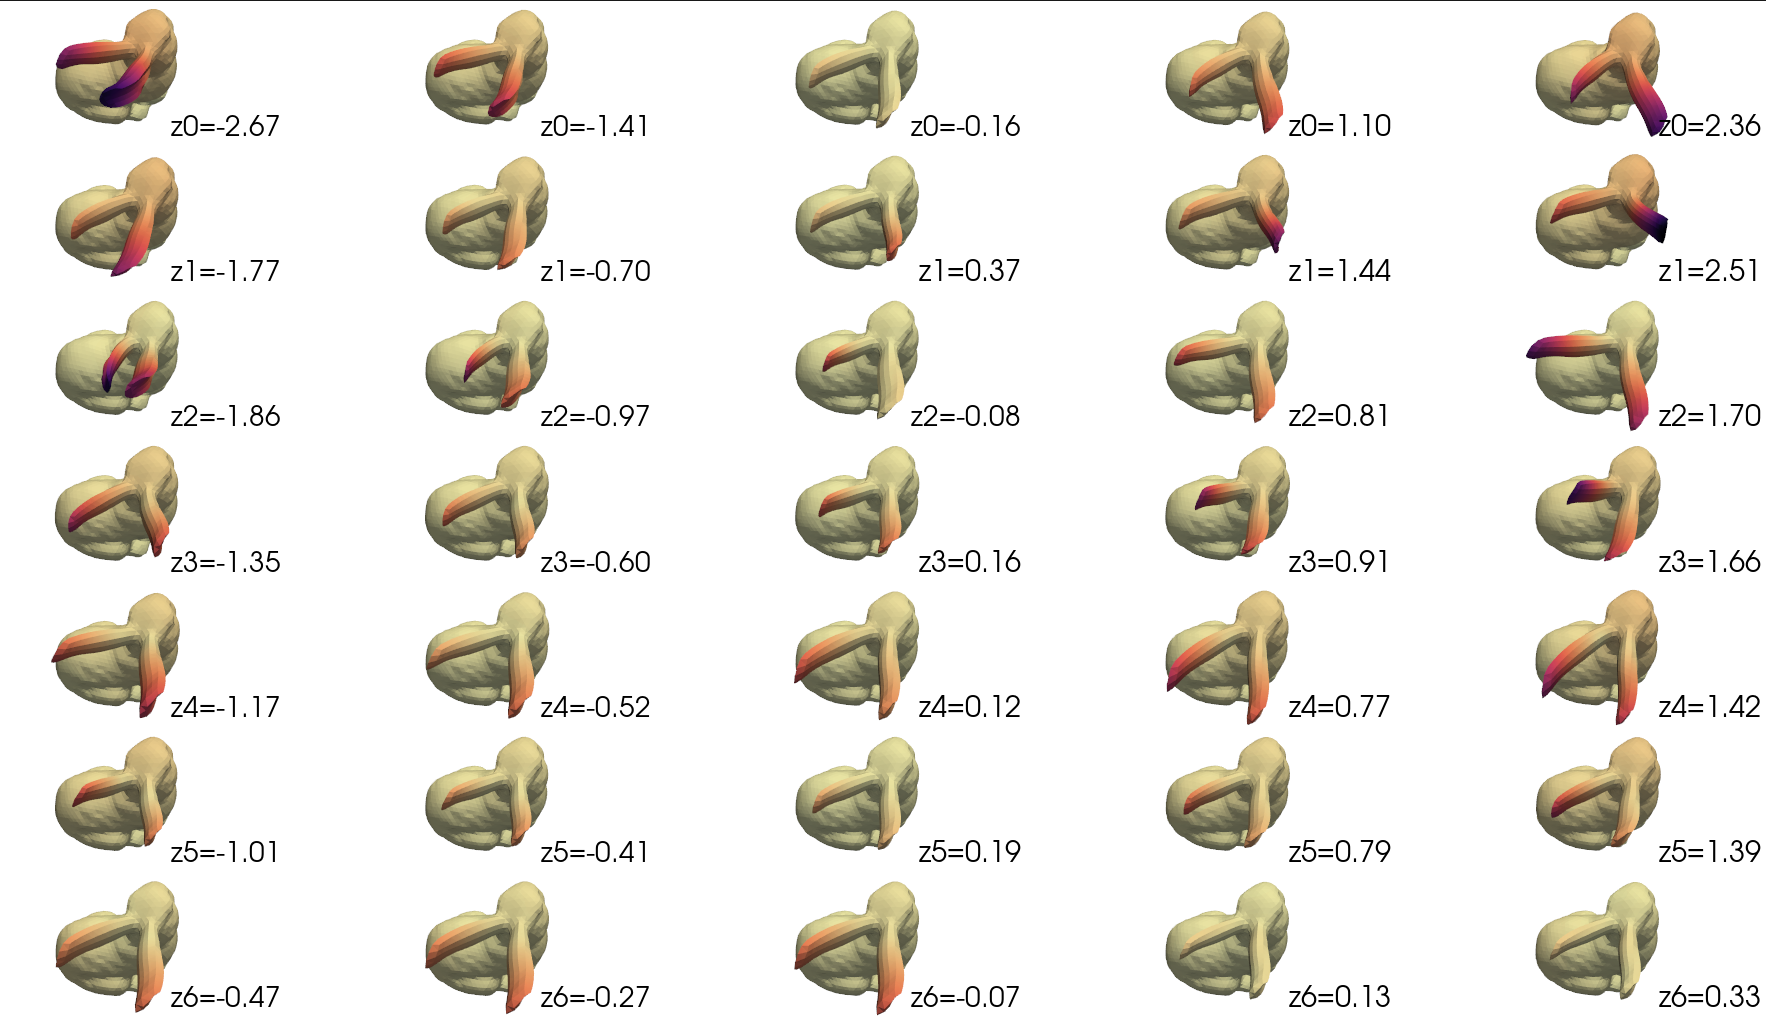
\includegraphics[width=\textwidth]{Images/latent_space_viz.png}
                \caption{Visualization of the learned corrections for the 7 modes of the Stanford Bunny.}
            \end{figure}
        \end{column}
    \end{columns}
\end{frame}

\begin{frame}{Dynamic Validation: A More Challenging Test}
    \frametitle{Dynamic Validation: A More Challenging Test}
    
    We tested the model's predictive capability over time, initializing with two FEM steps and then letting the model run.
    
    \begin{block}{Key Finding: Physical Plausibility over Positional Accuracy}
    While positional accuracy (MSE) degrades over time for all reduced models, our Neural Modes model shows a crucial advantage in maintaining physical realism.
    \end{block}
    
    \begin{columns}[T]
        \begin{column}{0.5\textwidth}
            \textbf{Displacement Error (MSE)}
            \begin{itemize}
                \item The MSE of our NM model is only slightly better than the Linear Modes model.
                \item Both models drift from the ground truth over a long simulation.
            \end{itemize}
            \begin{figure}
                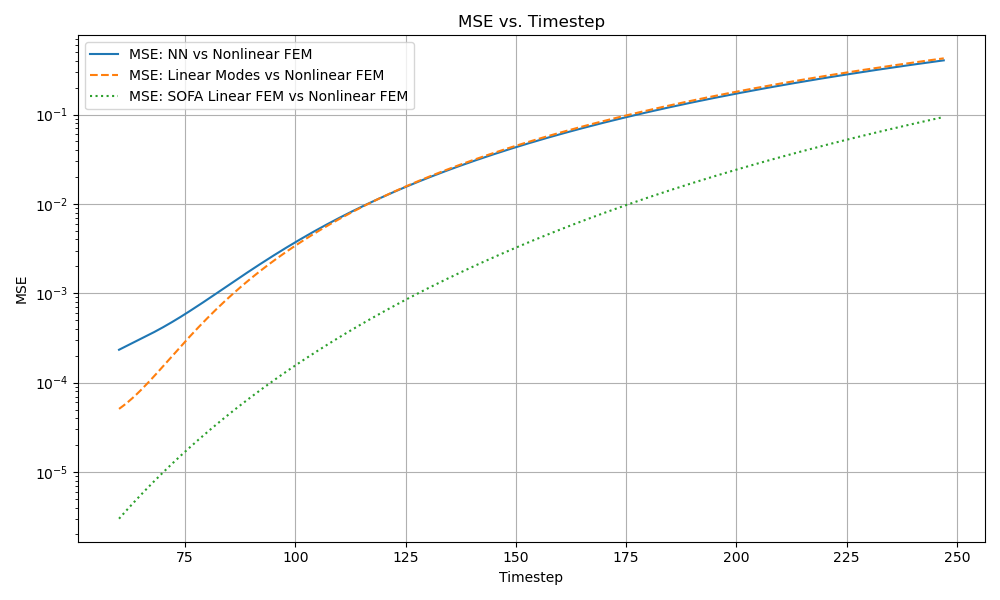
\includegraphics[width=\textwidth]{Images/beam_dynamic_mse.png}
            \end{figure}
        \end{column}
        
        \begin{column}{0.5\textwidth}
            \textbf{Internal Energy}
            \begin{itemize}
                \item \textbf{This is the key result.} The energy of the Linear Modes model explodes, a classic failure of linear models in nonlinear dynamics.
                \item Our \textbf{NM model's energy remains bounded and close to the ground truth}, producing a stable and physically plausible simulation.
            \end{itemize}
            \begin{figure}
                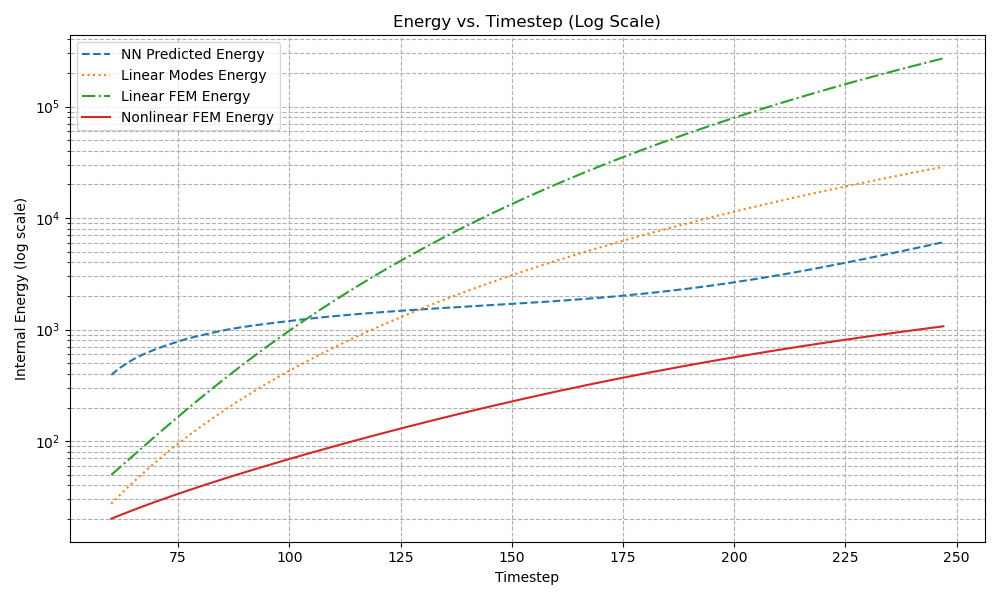
\includegraphics[width=\textwidth]{Images/beam_dynamic_energy.png}
            \end{figure}
        \end{column}
    \end{columns}
\end{frame}

\begin{frame}{Summary of Results}
    \frametitle{Summary of Results}
    
    \begin{itemize}
        \item \textbf{Supervised learning is essential:} A data-free, self-supervised approach was insufficient for this problem.
        \vspace{1.5em}
        
        \item \textbf{Excellent Static Accuracy:} In static tests, our Neural Modes model is up to an \textbf{order of magnitude more accurate} than linear models for large, nonlinear deformations.
        \begin{itemize}
            \item This holds for both simple (beam) and complex (bunny) geometries.
        \end{itemize}
        \vspace{1.5em}
        
        \item \textbf{Physically Plausible Dynamics:} In dynamic simulations, while positional accuracy eventually drifts, our model maintains \textbf{stable and physically realistic internal energy}, avoiding the "explosion" characteristic of linear models.
        \vspace{1.5em}
        
        \item \textbf{Interpretability:} The framework allows us to visualize and understand the learned nonlinear corrections, which is a significant advantage over typical "black-box" neural networks.
    \end{itemize}
\end{frame}

\begin{frame}{Conclusion: Summary of Contributions}
    \frametitle{Conclusion: Summary of Contributions}
    
    We have successfully developed and validated a modified Neural Modes framework for simulating large, nonlinear deformations.
    
    \begin{itemize}
        \item \textbf{Identified Limitations:} We showed that the original data-free, self-supervised approach was insufficient for our large-deformation use case.
        \vspace{1em}
        
        \item \textbf{Proposed a Supervised Method:} Our key contribution is a supervised training strategy that:
        \begin{itemize}
            \item Requires only a small amount of FEM simulation data.
            \item Uses a physics-informed loss function (blending displacement data with energy constraints).
            \item Achieves up to an order of magnitude greater accuracy than linear models in static, nonlinear regimes.
        \end{itemize}
        \vspace{1em}
        
        \item \textbf{Enabled Real-Time Performance:} By drastically reducing dimensionality (from thousands of DOFs to \textasciitilde{}7 modes), our method makes high-fidelity simulation feasible for interactive applications.
    \end{itemize}
\end{frame}

\begin{frame}{Limitations and Future Work}
    \frametitle{Limitations and Future Work}
    
    \begin{block}{Current Limitation: Dynamic Accuracy}
        While our dynamic simulations are physically plausible (conserving energy), the displacement accuracy drifts over long time horizons. This is likely due to error accumulation from the step-by-step optimization solver (L-BFGS).
    \end{block}
    
    \begin{alertblock}{Promising Future Direction: Fully Reduced Dynamics}
        Instead of optimizing at each time step, a more robust approach would be to solve a reduced system of equations directly in the modal space.
        
        \begin{itemize}
            \item Project the system matrices onto the modal basis:
            \begin{equation*}
                \left[M\right] = \left[\Phi\right]^T M \left[\Phi\right], \quad \left[K\right] = \left[\Phi\right]^T K \left[\Phi\right]
            \end{equation*}
            
            \item Solve the much smaller system of ODEs for the modal coordinates \(\mathbf{q}\):
            \begin{equation*}
                \left[{M}\right] \ddot{\mathbf{q}} + \left[{K}\right] \mathbf{q} = \mathbf{f}
            \end{equation*}
        \end{itemize}
        This would eliminate optimization errors and allow for more stable numerical integration, likely improving long-term accuracy significantly.
    \end{alertblock}
\end{frame}

\begin{frame}{Final Remarks}
    \frametitle{Final Remarks: The Big Picture}
    
    This work represents a significant step toward bridging the gap between computational speed and physical accuracy in nonlinear mechanics.
    
    \begin{itemize}
        \item \textbf{Performance:} We achieved real-time simulation speeds by combining dimensionality reduction with a fast neural network.
        \vspace{1em}
        
        \item \textbf{Physical Consistency:} The physics-informed loss ensures that our model produces energetically stable and plausible results, avoiding the failures of purely linear models.
        \vspace{1em}
        
        \item \textbf{Interpretability:} By learning corrections to a known physical basis, our model avoids being a complete "black box" and provides insight into nonlinear behavior.
    \end{itemize}
    
    \begin{alertblock}{Key Takeaway}
        The Neural Modes framework demonstrates how machine learning can be used to \textbf{enhance and augment} established physical modeling principles, rather than simply replacing them, paving the way for a new class of hybrid simulation tools.
    \end{alertblock}
\end{frame}

%bibliography
\begin{frame}[allowframebreaks]{References}
    \printbibliography[heading=none]
\end{frame}


\end{document}

